Abarcaré la posición de Jorge A. Sábato principalmente desde su artículo más conocido con Natalio Botana: \textit{La ciencia y
la tecnología en el desarrollo futuro de América Latina}.

En dicho artículo, los autores presentan un triangulo de relaciones (como el detallado en la Figura \ref{triangulo}) en el cual cada vertice
corresponde a un actor:
\begin{itemize}
    \item Gobierno: el conjunto de roles institucionales que tienen como objetivo formular políticas y movilizar recursos de y hacia los otros vértices a través de los procesos legislativo y administrativo.
    \item Infraestructura cientifico-tecnológica: el conjunto de sistemas educativos, institutos de investigación, academias de ciencias, etc.
    \item Estructura productiva: el conjunto de sectores productivos que provee los bienes y servicios que demanda una determinada sociedad.
\end{itemize}

\begin{figure}[H]
    \centering
    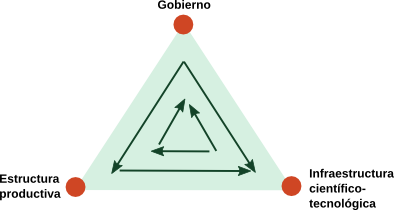
\includegraphics[width=0.6\textwidth]{imagenes/sabato.png}
    \caption{Triangulo de Sábato/Botana}\label{triangulo}
\end{figure}

% Luego, cada vertice tiene responsabilidades y se espera que se relacione con los demás de ciertas maneras.

En el artículo mencionado, Sábato habla de autonomía como la capacidad de decisión propia, y menciona que esta es el resultado de un proceso deliberado de interrelaciones entre los vértices.

Entonces, las posturas de Sábato en cuanto a la relación entre autonomía tecnológica y
autonomía nacional se pueden analizar (¿quizás parcialmente?) desde las responsabilidades que plantea para los distintos vertices, junto con sus relaciones.
% Este proceso se establece a través del flujo de demandas que circulan en sentido vertical (gobierno - los otros dos vertices) y en sentido horizantal.

Sábato distingue tres tipos de relaciones posibles:

\begin{itemize}
    \item \textit{Intrarelaciones}: las que suceden entre los diferentes componentes de un mismo vértice.
    \item \textit{Interrelaciones}: las que suceden entre dos vertices de un mismo triangulo.
    \item \textit{Extrarelaciones}: las que suceden entre dos vertices de triangulos distintos.
\end{itemize}

De las \textbf{intrarelaciones}, basta mencionar que deben estructurarse con vista a garantizar una determinada \textit{capacidad} para generar, incorporar o transformar demandas en un producto final que es la innovacion cientifico-tecnologica. En particular:

% Si hablamos de relaciones internas dentro de cada vertice, \textit{intrarelaciones}, éstas tienen por objetivo transformar a estos centros de convergencia
% en centros capaces de generar, incorporar y transformar demandas en un producto final que es la innovacion cientifico-tecnologica. Es decir:

\begin{enumerate}
    \item El vertice-gobierno requiere la capacidad para realizar una \textit{acción deliberada} en el ambito de políticas cientifico-tecnologicas, con el fin de formular un cuerpo de doctrina, de principios y estrategias capaces de fijar metas posibles, cuyo logro depende de una serie de decisiones politicas, de la asignación de recursos y de la programación cientifico-tecnologica.
    \item El vertice-infraestructura cientifico-tecnologica requiere la \textit{capacidad creadora}: un cientifico mediocre producirá ideas mediocres, por más dinero que se les inyecte.
    \item El vertice-estructura productiva requiere \textit{capacidad empresarial}, publica o privada, que si las definiremos según las ideas desarrolladas por Schumpeter, como aquella función que ``consiste en reformar o revolucionar el sistema de produccion, explotando un invento o, de manera más general, una posibilidad técnica no experimentada para producir una mercancía nueva o una mercancía antigua por un método nuevo, para abir una nueva fuente de previsión de materias primas o una nueva salida para los productos, para reorganizar una industria, etc''.
\end{enumerate}

ALGUNA CONCLUSION MÁS ?
Este segundo item está fuertemente relacionado con las ideas de Bayer de que las politicas tecnologicas deben buscar explotar las potencialidades existentes.

\vspace{0.5em}

En cuanto a las \textbf{interrelaciones}, Sábato les asigna una responsabilidad mayuscula: la generación de una capacidad de decisión propia en el campo cientifico-tecnológico es el \textit{resultado de un proceso deliberado de interrelaciones} entre el vertice-gobierno, el vertice-infraestructura cientifico-tecnologica y el vertice-estructura productiva.

Además, Sábato señala que el vértice de la infraestructura cientifico-tecnologica depende vitalmente de la acción deliberada del gobierno, entendido en un sentido muy amplio, sobre todo en lo que se refiere a asignación de recursos. Sin embargo, el vertice-gobierno juega tambien el papel de centro impulsor de demandas hacia la infraestructura cientifico-tecnologica, y es aquí donde reside la dificultad mayor en el modo como se concebirá la formulación de programas una vez tomada la decisión política.

\vspace{0.5em}

A continuación Sábato pasa a analizar las \textbf{extrarelaciones}.

En una sociedad donde funciona el triángulo de relaciones, las aperturas que se realicen hacia el exterior en materia de exportación de ciencia y tecnología original o de adaptación de tecnología importada, producen beneficios reales, ya sea a corto o largo plazo.

Muy distinto es cuando estas aperturas se realian entre vertices aislados con un triangulo plenamente desarrollado. Este problema es muy caracteristico de las sociedades latinoamericanas, y explica un sin fin de prolemas, como por ejemplo el éxodo de talentos. Mientras en nuestras sociedades el cientifico se encuentra desvinculado y aislado frente al gobierno y a la estructura productiva, en el nuevo lugar de trabajo, al cual lo conduce su exilio cultural, está automaticamente amparado por instituciones o centros de investigación que, a su vez, se encuentran insertos en el sistema de relaciones planteado.

\vspace{0.5em}

Habíendo dicho esto, Sábato afirma que en América Latina no existe un sistema de relaciones como el mencionado, ni tampoco hay conciencia acerca de la necesidad impostergable de establecerlo, por lo que hay una doble exigencia para las naciones en vías de desarrollo que busquen alcanzar su autonomía:
\begin{itemize}
    \item Crear una conciencia global para que nuestras sociedades asuman este problema en sus dimensiones reales.
    \item Actuar eficazmente sobre aquellos sectores en los cuales se podrían optimizar los recursos escasos en función del sistema de relaciones perseguido.
\end{itemize}

Además, Sabáto reafirma: corresponde al sector gubernamental formular una política tendiente a \textit{acoplar} la infraestructura cientifico-tecnologica al proceso de producción, ya sea creando los centros que así lo permitan o relacionando los centros ya existentes.

\vspace{0.5em}

Por último, quisiera dar un ejemplo concreto que presenta Sábato en su artículo \textit{Empresas y fábricas de tecnología}, de la creación en 1971 de una empresa Argentina estatal que responde a necesidades de desarrollo existentes en ese momento, la \textit{Empresa Nacional de Investigación y Desarrollo Eléctrico S.A.} (\texttt{ENIDE}). Su objetivo fundamental estaba definido en su estatuto como ``Producir, distribuir, comprar, vender, exportar, importar e intercambiar conocimiento técnico-científico en el campo de la energía eléctrica y sus aplicaciones'', y su creación obedecía a diversas circunstancias:

\begin{itemize}
    \item La existencia de un mercado importante y en rápido crecimiento.
    \item En el campo de la energía eléctrica, la Argentina era neto importador de tecnología.
    \item Existía capacidad científico-tecnológica apta para la producción de tecnología eléctica. La demanda interna era, sin embargo, muy escasa y de poca significación cualitativa.
    \item Por tratarse de un tipo de actividad que tenía poca tradición en el país, sobre cuya necesidad no existía aún conciencia clara y que requería capital de riesgo, sólo el Estado estaba en condiciones de ponerla en marcha.
\end{itemize}

% Notas Sábato:
% - no al colonialismo mental
% - pensar el desarrollo tecnologico como motor del desarrollo social y economico del país.
% - solo mediante ese manejo autonomo tecnologico podra una nacion comenzar a marchar
%     en la dirección que eventualmente le permitira disponer en cada caso de la tecnologia más ajustada
%     a sus propios objetivos, más respestuosa de su acervo cultural, más conveniente para sus propias
%     necesidades y más adecuadas a sus dotaciones de recursos y factores.
%
% - tecnologia nacional: manejar la tencologia como mas le convenga al país,
% - ¿Qué desarrollar y que comprar ? A veces conviene desarrollar primero, para luego importar en mejores condiciones.
% - La relacion entre politica tecnologica y economica, es determinante.
% - En particular, el uso del poder de compra del estado es el instrumento más importante
%
% - se va a alcanzar autonomia tecnologica: no como autonomia que reniega de la participacion de tecnologica extranjera,
%     sino como capacidad tecnologica autonoma, de generacion de tecnologia y de incorporacion de tecnologia estranjera a modo de configuracion de paquetes.
%     Lo contrario sería la desagregacion de paquetes tecnologicos, es decir: una participacion de componentes nacionales.
%
% - dependencia tecnologica: incorporación sumisa de las tecnologías disponibles por razones de disponibilidades y precios en el mercado.
% - autonomia: capacidad de desarrollo local: construir el triangulo, interrelacinando los tres vertices. Solo puede pasar si el estado tiene
%     una participacion clave en la estructura productiva.
% - presidente de SERBA: Empieza identificando cuales son los productos en los cuales puede haber desarrollo
%     tecnologico local y en los cuales podíamos prescindir de componentes importados.
% - Industrialización sustitutiva de importaciones.
% - Regimenes de promocion del desarrollo industrial, bastante protectivos: proteger a la industria naciente.
% - De vuelta: el compre nacional es un factor clave para la autonomia tecnologica, muestra una preferencia en cuanto proveedores externos.
% - Regulación de transferencia de tecnología extranjera
%
% -Por tanto, la desagregación tecnológica es también un instrumento de política industrial que busca maximizar
% la participación propia en la ejecución de proyectos de inversión por medio del incremento del componente tecnológico
%  nacional en la producción de un bien o de un servicio. Para eso es preciso investigar, en detalle, los agregados humanos,
%   económicos y técnicos de cada uno de los proyectos de inversión.

% http://www.fundacionsadosky.org.ar/seminario-ciencia-y-tecnologia-en-el-pensamiento-de-jorge-sabato-oscar-varsavsky-y-amilcar-herrera/
